\documentclass{article}
\usepackage[utf8]{inputenc}
\usepackage{amsmath}
\usepackage{setspace}
\usepackage{mathtools}
\usepackage{amssymb}
\usepackage{amsfonts}
\newcommand\der[2]{\frac{\partial{#1}}{\partial{#2}}}
\usepackage{sectsty}
\usepackage[parfill]{parskip}
\usepackage{changepage}   % for the adjustwidth environment
\usepackage{graphicx}
\graphicspath{ {./Pictures/} }
\usepackage{float}
\usepackage[margin=1in]{geometry}
\setlength{\parindent}{0em}
\sectionfont{\fontsize{12}{12}\selectfont}
\nonfrenchspacing
\renewcommand{\baselinestretch}{1.5}
\usepackage{indentfirst}
\usepackage{enumitem}
\setlist[itemize]{topsep=0pt,itemsep=0pt,partopsep=0pt,parsep=0pt}
\usepackage{xcolor}
\usepackage{titlesec}
\DeclareUnicodeCharacter{2212}{-}
\usepackage{tikz}
\usetikzlibrary{calc}
\newcommand{\tikzmark}[1]{\tikz[overlay,remember picture] \node (#1) {};}
\titleformat{\section}[block]{\color{blue}\Large\bfseries\filcenter}{}{1em}{}
\usepackage[normalem]{ulem}
\usepackage{calrsfs}
\renewcommand{\labelitemiv}{$\circledast$}
\renewcommand{\labelitemii}{$\circ$}
\titlespacing*{\subsection}{0pt}{0ex}{0ex}
\setlength{\parskip}{0.6em}

\title{ECON3510 Tutorial 9 Answers}
\date{2019}

\begin{document}

\maketitle

\section{Useful Formulas}

\begin{gather*}
  Q_{S} = Q_{D} \\
  CS = (C_{NG} \cdot Q_{D})/2 \\
  PS = P \cdot S_{NS} + [(Q_{S} - S_{NS}) \cdot P]/2
\end{gather*}

where $C_{NG}$ is the difference between $P$ at $Q_{D}=0$ and the actual $P$ \\
where $S_{NS}$ is just the quantity supplied at $P=0$


\section{Exercise 1}
\vspace{6mm}
\subsection{Question 1}

\begin{gather*}
  Q_{S} = Q_{D} \\
  100 + 40P = 400 - 10P \\
  50P = 300 \\
  \therefore P = 6 \\
  \therefore Q = 400 - 10(6) = 340
\end{gather*}

\par \vspace{0.8em}
\subsection{Question 2}

\begin{gather*}
  P = 4 \\
  \therefore Q_{S} = 100 + 40(4) = 260 \\
  \therefore Q_{D} = 400 - 10(4) = 360
\end{gather*}
The amount imported is:
\begin{gather*}
  I = Q_{D} - Q_{S} = 360 - 260 = 100
\end{gather*}
The consumer surplus is $CS = (C_{NG} \cdot Q_{D})/$ where $C_{NG}$ is the difference between $P$ at $Q_{D}=0$ and the actual $P$
\begin{gather*}
  Q_{D} = 0 = 400 - 10P \\
  \therefore P_{0} = 40 \\
  C_{NG} = P_{0} - P = 40 - 4 = 36
\end{gather*}
Using the consumer surplus formula:
\begin{gather*}
  CS = (36 \cdot 360)/2 = 6480
\end{gather*}
The intuition for the consumer surplus formula comes from the following image \\
\begin{center}
  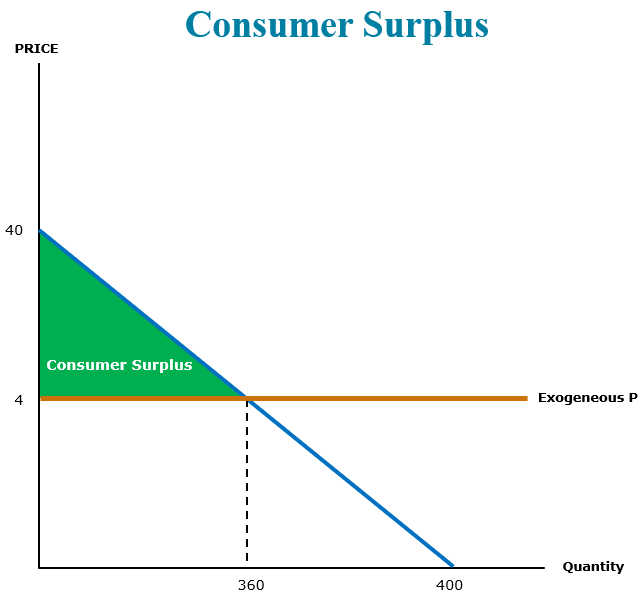
\includegraphics[width=8cm, height=8cm]{pic8}
\end{center}
The producer surplus is $PS = P \cdot S_{NS} + [(Q_{S} - S_{NS}) \cdot P]/2$ where $S_{NS}$ is the amount supplied at $P=0$
\begin{gather*}
  S_{NS} = 100 + 40(0) = 100
\end{gather*}
Therefore the producer surplus is:
\begin{gather*}
  PS = 4 \cdot 100 + [(260-100) \cdot 4]/2 = 720
\end{gather*}
The intuition for the producer surplus formula comes from the following image \\
\begin{center}
  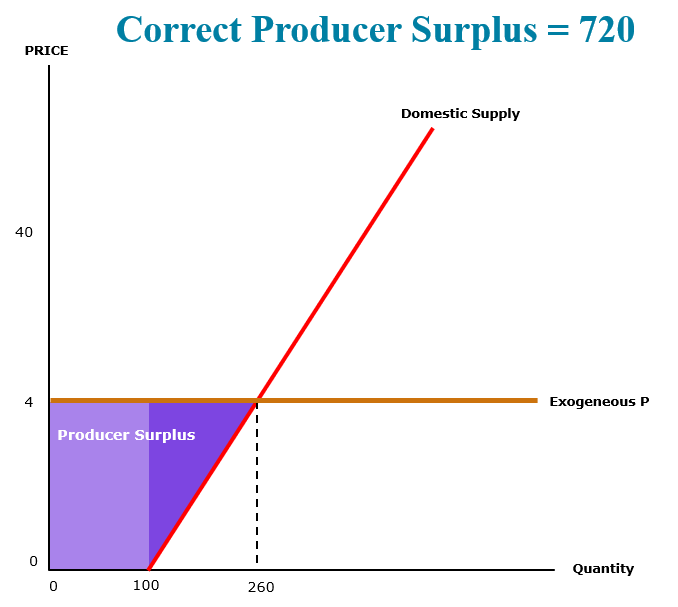
\includegraphics[width=8cm, height=8cm]{pic9}
\end{center}
Note that this is an unusual supply function since at $P=0$ we still have $Q>0$. Make sure that if calculating producer surplus graphically instead of using the formula that you calculate it using only the domestic supply and not the total supply, this will lead to the following incorrect results
\begin{center}
  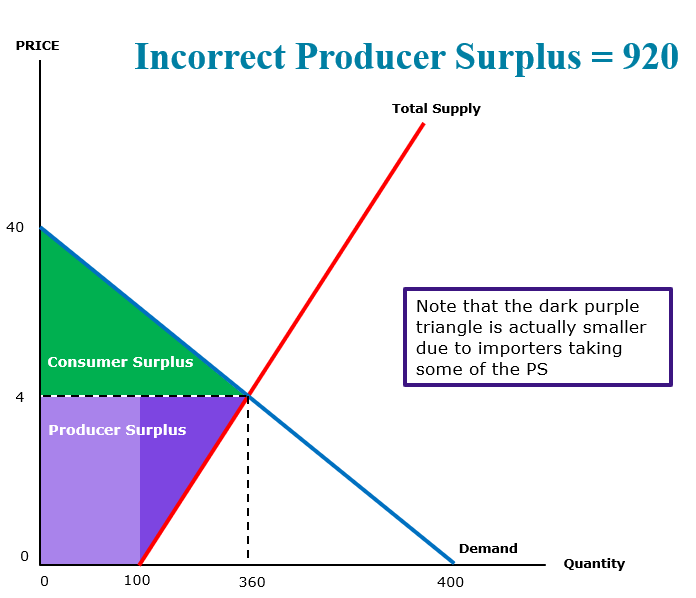
\includegraphics[width=8cm, height=8cm]{pic10}
\end{center}

\par \vspace{0.8em}
\subsection{Question 3}

Similar to question 2, just repeat using $P=5$ instead of $P=4$ and compare the two outcomes. \\
\begin{gather*}
  P = 5 \\
  \therefore Q_{S} = 100 + 40(5) = 300 \\
  \therefore Q_{D} = 400 - 10(5) = 350 \\
  \therefore I = Q_{D} - Q_{S} = 350 - 300 = 50 \\
  C_{NG} = P_{0} - P = 40 - 5 = 35 \\
  \therefore CS = (C_{NG} \cdot Q_{D})/2 = (35 \cdot 350)/2 = 6125 \\
\end{gather*}
So consumer surplus has fallen by 6480 - 6126 = 355 \\
Note that $S_{NS}$ has not changed and it is still 100 so producer surplus is:
\begin{gather*}
  PS = P \cdot S_{NS} +  [(Q_{S} - S_{NS}) \cdot P]/2 = 5 \cdot 100 +[(300 - 100) \cdot 5] /2  = 1000 \\
\end{gather*}
So producer surplus has actually increased by 1000-720 = 280 \\
The revenue from tariff is $I \cdot tariff = 50 \cdot 1 = 50$. \\
Total welfare reducion is just the sum of gains$^{-1}$ and losses$^{-1}$ as a result of the tariff (i.e. comparing Q2 and Q3) and so we have
\begin{gather*}
  Welfare \ Reduction = \Delta CS - \Delta PS - \Delta Revenue = 355 - 280 - 50 = 25
\end{gather*}
Note that if we were to have a fall in producer surplus and a increase in consumer surplus then we would rewrite this as:
\begin{gather*}
  Welfare \ Reduction = \Delta PS - \Delta CS - \Delta Revenue
\end{gather*}

\section{Exercise 2}
\vspace{6mm}
\subsection{Question 1}

\begin{gather*}
  Q_{SE} = Q_{DI} \\
  -120 + 40 P_{w} = 120 - 20 P_{w} \\
  60 P_{w} = 240 \\
  \therefore P_{w} = 4 \\
  \therefore Q_{DI} = 40
\end{gather*}

\par \vspace{0.8em}
\subsection{Question 2}


We now have the importer facing $P = P_{w} + 1.5$ and so for the importers equation $Q_{DI}$ we substitute in $P$:
\begin{gather*}
  Q_{SE} = Q_{DI} \\
  -120 + 40 P_{w} = 120 - 20 (P_{w} + 1.5) \\
  60 P_{w} = 210 \\
  P_{w} = 3.5
\end{gather*}
Note that $P_{w}$ is the world price but due to the tariff of 1.5 the US actually faces a price of $P=5$. Therefore we have the quantity imported in the US being:
\begin{gather*}
  Q_{DI} = 120 - 20(5) = 20
\end{gather*}
Tariff revenue is $R = tariff \cdot Q_{DI} = 1.5 \cdot 20 = 30$

\end{document}
